\section{Experiment}

We performed a between-subjects online experiment with young adults. %Participants were randomly assigned to one of two conditions: MindMargin or the vertical commenting interface.

\minisubsection{Participants}
106 online participants landed on our page for our user study and evaluation, of which 46 proceeded to begin and complete the study (30 female). 19 participants were randomly assigned to the Mind Margin condition and 27 to the vertical interface condition.  Participants were recruited online through social media and college listservs. Participants were college students, aged 18 to 25, and 68\% hailed from the local university. The self-reported reading frequency of online news among participants ranged from daily to almost never. 

\minisubsection{Experimental Conditions}
The two conditions in our study were MindMargin and the traditional vertical interface. The article was selected on the basis of its opinionated nature and its relevance both in recent news and to our anticipated participant pool. We chose an opinion piece from our university's undergraduate publication, titled ``Don't Teach for America.''. Teach For America (TFA) is a non-profit organization that recruits recent college graduates to teach for two years in public schools. 

The article already had over fifty comments by affiliates and non-affiliates of the university alike, from which we selected the top 39 comments as ranked by Disqus, the existing commenting system on the publication's website, to be used in our study. The same comments were used in both conditions. In the traditional vertical interface, the comments appeared in the identical order as ranked in the original article. In MindMargin, we anchored them to the article based on textual references, specific phrases, quotes, and relevant content in each comment. 

%Users could make new comments by writing in the static new comment box above existing comments in the traditional interface and by clicking any part of the article to open a new comment box in MindMargin. In the MindMargin condition, we provided participants with simple, temporary instructions: "click the text to comment."

%XXXX include that last paragraph? XXXX

\minisubsection{Tasks}
To ensure that our results would be informative for the design of real-world commenting systems, we designed the experimental tasks to focus participants' attention on the content of the article.  The study design did not emphasize that the evaluation of the commenting system was the object of the study, but this information was clearly communicated and disclosed in the consent form. 

Participants were presented with an article and they were instructed to read the article and to anticipate a questionnaire that followed, but were not asked or required to interact with the commenting system.  Once they completed reading the article, we asked them the general stance of the article -- For TFA or Against TFA -- and, in a free-text response, we requested two pieces of supporting evidence used in the article to verify their reading and comprehension of the article. All 46 participants gave correct and thorough answers to these verification questions. Participants were then asked to complete a post-experiment questionnaire (see Figure \ref{fig:questionnaire}), which asked for their personal stance on the issue, whether they liked the article, and whether they agreed with the article. They were also asked to self-report whether they read the comments in the article and to provide two adjectives that described either their reaction to, or a description of, the comments.

\marginpar{
\begin{figure}
  \begin{center}
  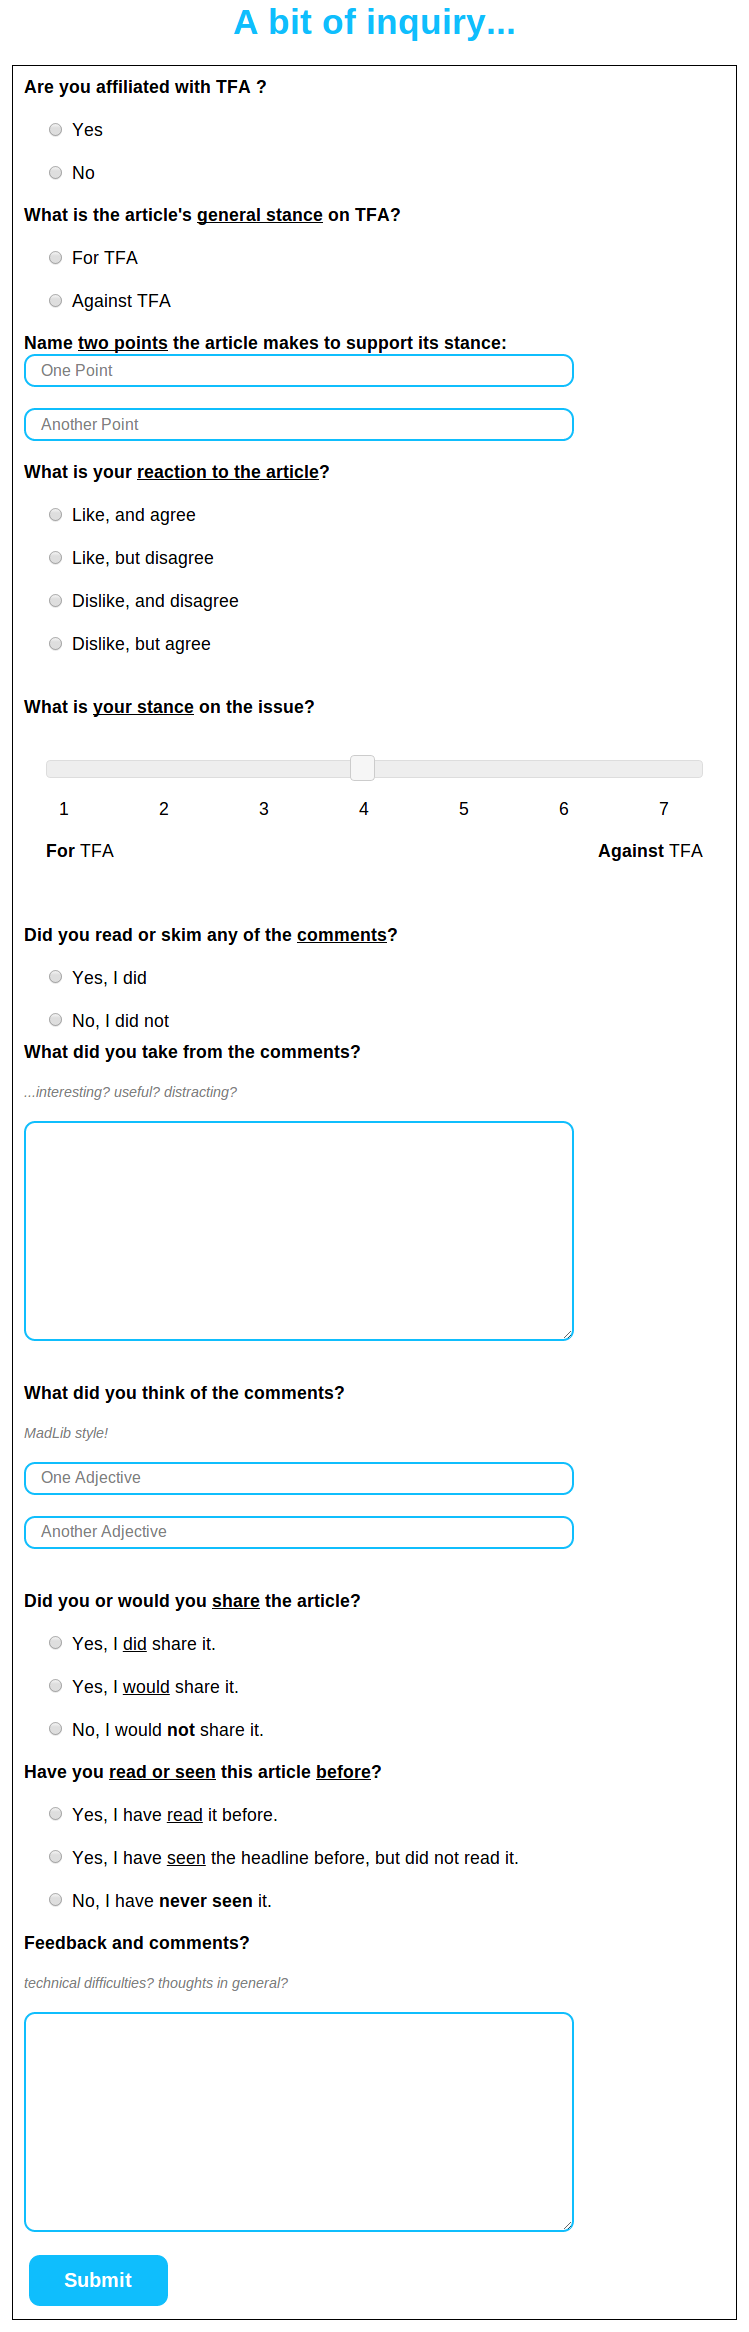
\includegraphics[width=\marginparwidth]{q1.png}
  \caption{The post-experiment questionnaire for validation and stance quantification.}
  \label{fig:questionnaire}
  \end{center}
\end{figure}
}

%and were not permitted to refer back to the article once the questionnaire was administered. These questions included the following: [[XXX list questions in questionnaire -- KZG: or at least summarize the purpose of the questionnaire. Oh, here's a trick: you can make the questions into a figure and post them on the margin.]]

To further incentivize participants to focus on the content of the article and reflect on the issue discussed therein, we used the following tagline to advertise the study: ``Do you (really) think like a Harvard student?'' and at the completion of the study, we provided them with feedback comparing their answers to the responses made by other Harvard students.

%In order to reproduce the conditions under which one would normally read a news article, we chose to recruit participants online and to allow them to self-select themselves into reading the article based on personal time and interest. In order to motivate our participants to actually read or skim the article, instead of skip it, we chose not to use monetary or other time-sensitive incentives. Instead, we chose to design the experiment around the survey question, "Do you (really) think like a student [from our local university]?" 
%
%We then asked participants follow-up questions to verify that they read the article, which included both the overall stance of the article and, in a free-text response, two pieces of supporting evidence used in the article. All 46 participants gave correct and thorough answers to these verification questions. Participants were then asked to complete a post-experiment questionnaire and were not permitted to refer back to the article once the questionnaire was administered.

\minisubsection{Procedure}
Participants were given an initial questionnaire asking basic demographics and news reading frequency. Before being shown the article, they were also asked either to provide a username or pseudonym, or to remain anonymous. Participants were allotted 10 minutes to read the article. After 2 minutes, they were permitted to proceed to the questionnaire. The 2-minute delay was to ensure the reading of the article, and did not seem to prevent fast readers from moving too slowly, as the average reading time was 3 minutes 47 seconds. 

%In the follow-up questionnaire, reading verification questions were first posed. Participants were then asked their personal stance on the article, whether they liked the article, and whether they agreed with the article. They were also asked to self-report whether they read the comments in the article and to provide two adjectives that described either their reaction to, or a description of, the comments.

\minisubsection{Design and Analysis}
We used a between-subject full factorial design with two factors and the interaction between them.

The two factors were: {\it Prototype} \{``mindmargin`` for the new horizontal interface MindMargin or ``regular`` for the traditional vertical interface\}, and {\it Prior exposure to the article} \{``read`` if they have read or skimmed the article before, ``seen`` if they have seen the article but did not read or skim it, and ``none`` if they have neither read nor seen the article previously\}. To compare conditions, we excluded 9 participants who reported not to have read the comments (5 MindMargin). In addition to commenting system design, there was no significant difference in gender, reading frequency, or other demographic information among excluded participants.

We analyzed two dependent variables.  First, we computed {\it Stance Polarization (SP)}, which captured how far a participant's personal stance on the issue (on a scale from 0-Strongly For TFA to 100-Strongly Against TFA) was removed from the neutral stance (50).%We excluded 2 participants who opted out of answering this question (1 MindMargin), both of whom were already excluded for having not read the comments.

% after reading and interacting with their respective commenting systems. We computed each participant's SP, or their Stance Polarization, by measuring the distance between their stance and a neutral stance of 50 as $|50 - stance|$. 

Second, we measured {\it Attitude Toward Comments (ATC)}.  As mentioned earlier, each participant who reported having read the comments was asked to provide two adjectives describing their reaction to the comments accompanying the article.
%For our second hypothesis, we examined the two free-text responses describing either participants' reaction to the comments or their description of the comments, both in response to the question: ``What did you think of the comments from the article?`` 
We asked four independent raters, blind to the experiment, to classify these adjectives using a four-bin classifier (``Positive,`` ``Negative,`` ``Neutral,`` and ``Invalid``). %They were told to classify the adjectives provided that they were in answer to the free-text question, posed on the survey: ``What did you think of the comments (from article X)?`` 
We removed adjectives given two or more ``Invalid`` classifications. % as outliers, which only appeared in the vertical condition. 
For the remaining adjectives, we used the majority vote.  Disagreements among raters were never between ``Positive'' and ``Negative''.  
%We found that adjectives without uniform encoding observed an uncontradictory mix of classifications: ``Positive`` and ``Neutral`` or ``Neutral`` and ``Negative,`` but never ``Positive`` and ``Negative``. 
We were thus confident in using the resulting median encodings for the final classification of the specified adjectives.

\marginpar{
\begin{figure}
  \begin{center}
  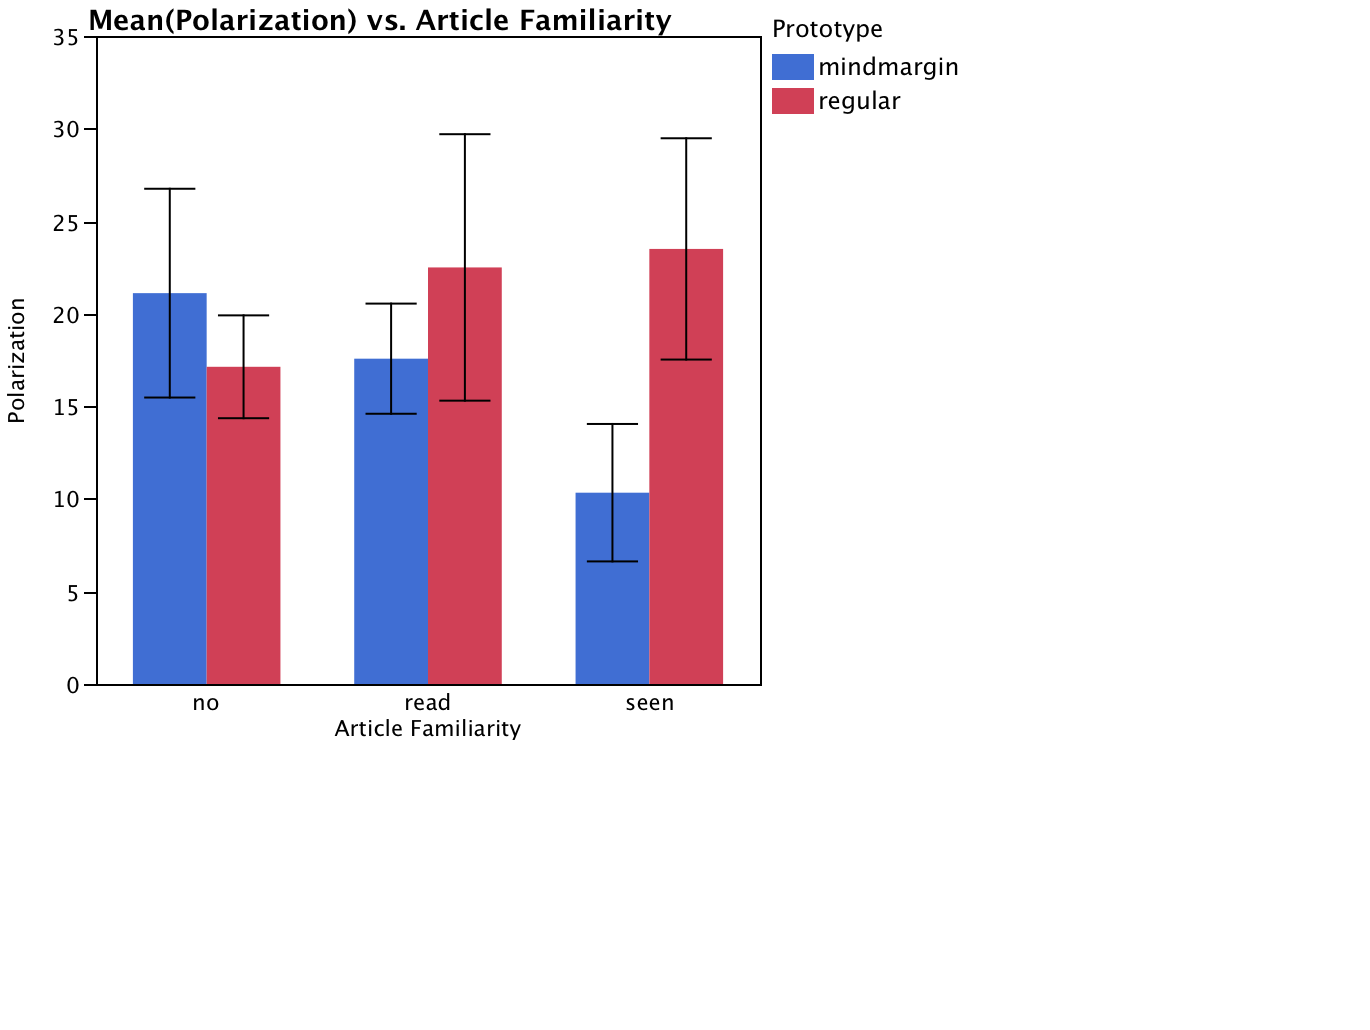
\includegraphics[width=\marginparwidth]{familiarity.png}
  \caption{When using MindMargin, participants with prior exposure to the article reported less extreme stance.}
  \label{fig:leastsqs}
  \end{center}
\end{figure}
}

\marginpar{
\begin{figure}
  \begin{center}
  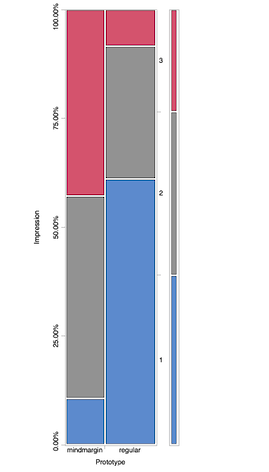
\includegraphics[width=\marginparwidth]{mosaicplot_revised6.png}
  \caption{When using MindMargin, the majority of participants described the comments as positive (3) rather than neutral (2) or negative (1).}
  \label{fig:mosaic}
  \end{center}
\end{figure}
}


We treated SP as a continuous variable and we analyzed it using analysis of variance.
We treated ATC as an ordinal variable and we analyzed it using ordinal logistic regression.

%we examined  the adjectives that participants who read the comments provided in reaction to the comment